% ══════════════════════════════════════════════
% CHƯƠNG 4 — THỰC THI KỸ THUẬT VÀ CÔNG NGHỆ
% Người viết: TV4 (API — Controllers, JWT, Swagger)
% ══════════════════════════════════════════════

\chapter{Thực thi Kỹ thuật và Công nghệ}

\section{ASP.NET Core Web API}\label{Sec4.1}

\subsection{Thiết kế RESTful Endpoints}\label{sub4.1.1}

\begin{de}\label{def4.1}
  REST (Representational State Transfer) là phong cách kiến trúc phần mềm
  dựa trên giao thức HTTP, trong đó mỗi tài nguyên được định danh bằng một URI
  duy nhất và được thao tác qua các HTTP verb chuẩn:
  \textbf{GET} (truy vấn dữ liệu),
  \textbf{POST} (tạo mới tài nguyên),
  \textbf{PUT} (cập nhật toàn bộ tài nguyên),
  \textbf{PATCH} (cập nhật một phần) và
  \textbf{DELETE} (xóa tài nguyên).
  Nguyên tắc đặt tên URL sử dụng \emph{danh từ số nhiều} để chỉ tập hợp
  tài nguyên (ví dụ: \texttt{/api/tours}, \texttt{/api/bookings}),
  không đặt động từ trong đường dẫn.
  Phản hồi kèm HTTP status code ngữ nghĩa:
  \texttt{200 OK}, \texttt{201 Created}, \texttt{204 No Content},
  \texttt{400 Bad Request}, \texttt{401 Unauthorized},
  \texttt{403 Forbidden}, \texttt{404 Not Found}, \texttt{409 Conflict}.
\end{de}


\begin{longtable}{|l|p{6cm}|p{4.2cm}|l|}
  \hline
  \textbf{Method} & \textbf{Endpoint} & \textbf{Mô tả} & \textbf{Quyền} \\
  \hline
  \endfirsthead
  \hline
  \textbf{Method} & \textbf{Endpoint} & \textbf{Mô tả} & \textbf{Quyền} \\
  \hline
  \endhead
  \multicolumn{4}{r}{\textit{(tiếp theo trang sau)}} \\
  \endfoot
  \hline
  \endlastfoot
  GET    & /api/tours                                     & Danh sách tour (pagination + filter)      & Public   \\ \hline
  GET    & /api/tours/\{id\}                              & Chi tiết tour                             & Public   \\ \hline
  GET    & /api/tours/search?dest=\&priceMin=\&priceMax=\&date= & Tìm kiếm nâng cao               & Public   \\ \hline
  POST   & /api/tours                                     & Thêm tour mới                             & Admin    \\ \hline
  PUT    & /api/tours/\{id\}                              & Cập nhật thông tin tour                   & Admin    \\ \hline
  DELETE & /api/tours/\{id\}                              & Xóa tour                                  & Admin    \\ \hline
  POST   & /api/bookings                                  & Đặt tour (sp\_CreateBooking)              & Customer \\ \hline
  GET    & /api/bookings/\{id\}                           & Chi tiết booking (vw\_BookingDetails)     & Auth     \\ \hline
  PUT    & /api/bookings/\{id\}/cancel                    & Hủy booking (sp\_CancelBooking)           & Customer \\ \hline
  GET    & /api/bookings/account/\{id\}                   & Lịch sử booking của tài khoản             & Auth     \\ \hline
  POST   & /api/auth/register                             & Đăng ký tài khoản mới                    & Public   \\ \hline
  POST   & /api/auth/login                                & Đăng nhập, nhận JWT token                 & Public   \\ \hline
  GET    & /api/accounts/\{id\}/profile                   & Xem hồ sơ cá nhân                         & Auth     \\ \hline
  PUT    & /api/accounts/\{id\}/profile                   & Cập nhật hồ sơ cá nhân                   & Auth     \\ \hline
  GET    & /api/employees                                 & Danh sách nhân viên / HDV                 & Admin    \\ \hline
  POST   & /api/employees                                 & Thêm nhân viên / HDV                      & Admin    \\ \hline
  PUT    & /api/employees/\{id\}                          & Cập nhật nhân viên / HDV                  & Admin    \\ \hline
  DELETE & /api/employees/\{id\}                          & Xóa nhân viên / HDV                       & Admin    \\ \hline
  GET    & /api/reports/revenue                           & Doanh thu theo tour (vw\_TourRevenue)     & Admin    \\ \hline
  GET    & /api/reports/popular-tours                     & Tour phổ biến (vw\_PopularTours)          & Admin    \\ \hline
  GET    & /api/reports/revenue-by-month                  & Doanh thu theo tháng (sp\_RevenueReport)  & Admin    \\ \hline
  GET    & /api/reports/occupancy                         & Tỷ lệ lấp đầy chỗ                         & Admin    \\ \hline
  GET    & /api/categories                                & Danh sách loại hình tour                  & Public   \\ \hline
  GET    & /api/destinations                              & Danh sách điểm đến                        & Public   \\ \hline
  POST   & /api/payments                                  & Ghi nhận thanh toán                       & Auth     \\ \hline
  GET    & /api/payments/booking/\{id\}                   & Lịch sử thanh toán theo booking           & Auth     \\ \hline
  POST   & /api/reviews                                   & Đăng đánh giá tour                        & Customer \\ \hline
  GET    & /api/export/tours/xml                          & Xuất tour ra XML (LINQ to XML)            & Admin    \\ \hline
  POST   & /api/import/tours/xml                          & Nhập tour từ XML                          & Admin    \\
  \hline
  \caption{Danh sách các RESTful Endpoints chính}\label{table:endpoints}
\end{longtable}

\subsection{Cấu trúc Controller}\label{sub4.1.2}

% [TV4] Chèn code C# của 1 Controller tiêu biểu, bao gồm ít nhất
% GET (list), GET (detail), POST, PUT, DELETE.

\begin{lstlisting}[style=csharp, caption={ToursController --- các action chính}]
[ApiController]
[Route("api/tours")]
[Produces("application/json")]
public class ToursController(ITourService svc) : ControllerBase
{
    // ── GET /api/tours?page=1&pageSize=10&cateId=&desId=&priceMin=&priceMax=
    //Danh sach tour — phan trang va loc theo danh muc, diem den, khoang gia
    //chi admin, staff moi duoc xem
    [HttpGet]
    [AllowAnonymous]
    [ProducesResponseType(typeof(ApiResponse<PagedResult<TourListDto>>), 200)]
    public async Task<IActionResult> GetAll(
        [FromQuery] int page = 1,
        [FromQuery] int pageSize = 10,
        [FromQuery] int? cateId = null,
        [FromQuery] int? desId = null,
        [FromQuery] decimal? priceMin = null,
        [FromQuery] decimal? priceMax = null)
    {
        if (page < 1 || pageSize < 1 || pageSize > 100)
            return BadRequest(ApiResponse<string>.Fail("page/pageSize không hợp lệ."));

        var result = await svc.GetToursAsync(page, pageSize, cateId, desId, priceMin, priceMax);
        return Ok(ApiResponse<PagedResult<TourListDto>>.Ok(result));
    }

    // ── GET /api/tours/search?destination=&priceMin=&priceMax=&date=
    //Tim kiem nang cao — goi sp_SearchTours qua ADO.NET
    [HttpGet("search")]
    [AllowAnonymous]
    [ProducesResponseType(typeof(ApiResponse<IEnumerable<object>>), 200)]
    public async Task<IActionResult> Search(
        [FromQuery] string? destination = null,
        [FromQuery] decimal? priceMin = null,
        [FromQuery] decimal? priceMax = null,
        [FromQuery] DateOnly? date = null)
    {
        var results = await svc.SearchToursAsync(destination, priceMin, priceMax, date);
        return Ok(ApiResponse<IEnumerable<object>>.Ok(results.Cast<object>()));
    }

    // ── GET /api/tours/popular
    //Tour pho bien — truy van vw_PopularTours
    [HttpGet("popular")]
    [AllowAnonymous]
    [ProducesResponseType(typeof(ApiResponse<IEnumerable<object>>), 200)]
    public async Task<IActionResult> GetPopular()
    {
        var results = await svc.GetPopularToursAsync();
        return Ok(ApiResponse<IEnumerable<object>>.Ok(results.Cast<object>()));
    }

    // ── GET /api/tours/{id}
    //Chi tiet tour — kem lich khoi hanh va diem danh gia trung binh
    [HttpGet("{id:int}")]
    [AllowAnonymous]
    [ProducesResponseType(typeof(ApiResponse<TourDetailDto>), 200)]
    [ProducesResponseType(typeof(ApiResponse<string>), 404)]
    public async Task<IActionResult> GetById(int id)
    {
        var tour = await svc.GetTourDetailAsync(id);
        if (tour is null)
            return NotFound(ApiResponse<string>.Fail($"Tour ID {id} không tồn tại."));

        return Ok(ApiResponse<TourDetailDto>.Ok(tour));
    }

    // ── POST /api/tours
    //Them tour moi — chi Admin
    [HttpPost]
    [Authorize(Roles = "Admin")]
    [ProducesResponseType(typeof(ApiResponse<TourDetailDto>), 201)]
    [ProducesResponseType(typeof(ApiResponse<string>), 400)]
    public async Task<IActionResult> Create([FromBody] TourRequestDto dto)
    {
        if (!ModelState.IsValid)
            return BadRequest(ApiResponse<string>.Fail("Dữ liệu không hợp lệ."));

        var created = await svc.CreateTourAsync(dto);
        return CreatedAtAction(nameof(GetById), new { id = created.TourId },
            ApiResponse<TourDetailDto>.Ok(created, "Tạo tour thành công."));
    }

    // ── PUT /api/tours/{id}
    //Cap nhat tour — chi Admin
    [HttpPut("{id:int}")]
    [Authorize(Roles = "Admin")]
    [ProducesResponseType(typeof(ApiResponse<TourDetailDto>), 200)]
    [ProducesResponseType(typeof(ApiResponse<string>), 404)]
    public async Task<IActionResult> Update(int id, [FromBody] TourRequestDto dto)
    {
        if (!ModelState.IsValid)
            return BadRequest(ApiResponse<string>.Fail("Dữ liệu không hợp lệ."));

        var updated = await svc.UpdateTourAsync(id, dto);
        return Ok(ApiResponse<TourDetailDto>.Ok(updated, "Cập nhật tour thành công."));
    }

    // ── DELETE /api/tours/{id}
    // Xóa tour (Chặn xóa nếu đã có khách đặt, xóa cứng nếu chưa có booking) — chi Admin
    [HttpDelete("{id:int}")]
    [Authorize(Roles = "Admin")]
    [ProducesResponseType(typeof(ApiResponse<string>), 200)]
    [ProducesResponseType(typeof(ApiResponse<string>), 404)]
    public async Task<IActionResult> Delete(int id)
    {
        await svc.DeleteTourAsync(id);
        return Ok(ApiResponse<string>.Ok("deleted", "Xóa tour thành công."));
    }
}
\end{lstlisting}

\section{Xác thực và Phân quyền (JWT + RBAC)}\label{Sec4.2}

\subsection{JWT Authentication}\label{sub4.2.1}

\begin{thm}\label{thm4.1}
  JSON Web Token (JWT) là cơ chế xác thực \emph{stateless}: toàn bộ thông tin
  định danh người dùng (AccountId, Email, danh sách Role) được ký số và mã hóa
  bên trong token bằng thuật toán HMAC-SHA256 cùng một khóa bí mật.
  Server không cần lưu trữ session; mỗi request chỉ cần xác minh chữ ký
  của token là đủ để nhận dạng danh tính và quyền hạn của người dùng.
\end{thm}

\noindent\begin{proof}
  Khi client gửi request kèm header \texttt{Authorization: Bearer <token>},
  ASP.NET Core JWT Middleware giải mã phần \emph{payload} (Base64Url)
  và kiểm tra chữ ký bằng đúng \texttt{SecretKey} đã cấu hình.
  Nếu chữ ký hợp lệ và token chưa hết hạn (claim \texttt{exp}),
  các claim --- bao gồm \texttt{Role} --- được nạp vào \texttt{ClaimsPrincipal}
  mà không cần một lần truy vấn cơ sở dữ liệu nào.
  Nhờ đó, hệ thống có thể scale ngang tự do vì mọi instance đều
  tự xác minh được token mà không cần chia sẻ trạng thái phiên.
  \QEDAa
\end{proof}
\begin{lstlisting}[style=csharp, caption={Cấu hình JWT trong Program.cs}]
// Program.cs
var jwtSection = cfg.GetSection("JwtSettings");
var secretKey = jwtSection["SecretKey"]!;

builder.Services.AddAuthentication(JwtBearerDefaults.AuthenticationScheme)
.AddJwtBearer(options =>
{
    var key = Encoding.UTF8.GetBytes( builder.Configuration["JwtSettings:SecretKey"]!);
    options.TokenValidationParameters =
        new TokenValidationParameters
        {
            ValidateIssuer = true,
            ValidateAudience = true,
            ValidateLifetime = true,
            ValidateIssuerSigningKey = true,
            ValidIssuer =builder.Configuration["JwtSettings:Issuer"],
            ValidAudience = builder.Configuration["JwtSettings:Audience"],
            IssuerSigningKey = new SymmetricSecurityKey(key)
        };
});

builder.Services.AddAuthorization();
\end{lstlisting}

\subsection{Phân quyền theo Role}\label{sub4.2.2}
Hệ thống định nghĩa ba Role lưu trong bảng \texttt{Roles} và gán qua
bảng trung gian \texttt{AccountRoles}: \textbf{Admin} (quản trị toàn hệ thống),
\textbf{Staff} (nhân viên --- chỉ xem) và
\textbf{Customer} (khách hàng --- thao tác cá nhân).
Phân quyền được khai báo trực tiếp bằng attribute
\texttt{[Authorize(Roles = "...")]} trên từng Controller hoặc Action.

\begin{table}[H]
  \begin{center}
    \begin{tabular}{|l|c|c|c|}
      \hline
      \textbf{Chức năng} & \textbf{Admin} & \textbf{Staff} & \textbf{Customer} \\
      \hline
      Xem danh sách / chi tiết tour         & \checkmark & \checkmark & \checkmark \\
      Tìm kiếm tour nâng cao                & \checkmark & \checkmark & \checkmark \\
      CRUD Tour                             & \checkmark &            &            \\
      CRUD Categories / Destinations        & \checkmark &            &            \\
      CRUD Employees (hướng dẫn viên)       & \checkmark &            &            \\
      Xem tất cả Booking                    & \checkmark & \checkmark &            \\
      Đặt tour                              &            &            & \checkmark \\
      Hủy booking của mình                  &            &            & \checkmark \\
      Xem booking cá nhân                   &            &            & \checkmark \\
      Đánh giá tour (cần Booking Completed) &            &            & \checkmark \\
      Ghi nhận thanh toán                   & \checkmark & \checkmark & \checkmark \\
      Xem báo cáo doanh thu                 & \checkmark &            &            \\
      Export / Import XML                   & \checkmark &            &            \\
      \hline
    \end{tabular}
  \end{center}
  \caption{Bảng phân quyền theo Role}\label{table:phanquyen}
\end{table}

\section{Global Exception Middleware}\label{Sec4.3}

Để tránh lặp lại khối \texttt{try-catch} ở từng Controller và đảm bảo
mọi exception không xử lý được đều trả về JSON chuẩn thay vì HTML stack trace,
hệ thống đăng ký \texttt{ExceptionMiddleware} ở đầu pipeline trong \texttt{Program.cs}.
Middleware bắt toàn bộ exception, ghi log, rồi ánh xạ sang HTTP status code
và thông điệp JSON đồng nhất theo kiểu \texttt{ApiResponse}.

\begin{lstlisting}[style=csharp, caption={ExceptionMiddleware xử lý lỗi tập trung}]
public class ExceptionMiddleware(RequestDelegate next, ILogger<ExceptionMiddleware> logger)
{
    public async Task InvokeAsync(HttpContext ctx)
    {
        try
        {
            await next(ctx);
        }
        catch (Exception ex)
        {
            logger.LogError(ex, "Unhandled exception: {Message}", ex.Message);
            await HandleExceptionAsync(ctx, ex);
        }
    }

    private static Task HandleExceptionAsync(HttpContext ctx, Exception ex)
    {
        ctx.Response.ContentType = "application/json";

        ctx.Response.StatusCode = ex switch
        {
            KeyNotFoundException => (int)HttpStatusCode.NotFound,
            UnauthorizedAccessException => (int)HttpStatusCode.Forbidden,
            InvalidOperationException => (int)HttpStatusCode.Conflict,
            ArgumentException => (int)HttpStatusCode.BadRequest,
            _ => (int)HttpStatusCode.InternalServerError
        };

        var body = JsonSerializer.Serialize(
         ApiResponse<string>.Fail(
             ex.InnerException?.Message ?? ex.Message),
         new JsonSerializerOptions
         {
             PropertyNamingPolicy = JsonNamingPolicy.CamelCase
         });

        return ctx.Response.WriteAsync(body);
    }
}

// Đăng ký trong Program.cs 
app.UseMiddleware<ExceptionMiddleware>();
\end{lstlisting}
\section{LINQ to XML --- Export và Import}\label{Sec4.4}

\begin{ex}\label{ex4.1}

  Hệ thống cung cấp tính năng xuất (\emph{Export}) và nhập (\emph{Import})
  dữ liệu tour dưới định dạng XML thông qua \texttt{XmlService} ở tầng BLL,
  được gọi từ các endpoint \texttt{GET /api/export/tours/xml} và
  \texttt{POST /api/import/tours/xml} (chỉ Admin).
  LINQ to XML (\texttt{System.Xml.Linq}) được dùng để xây dựng và phân tích
  cây \texttt{XDocument}/\texttt{XElement} thuần túy, không phụ thuộc ADO.NET hay EF Core.
  Tính năng này hỗ trợ sao lưu danh mục tour và trao đổi dữ liệu
  với các hệ thống bên ngoài.
\end{ex}

% [TV4] Chèn code Export XML
\begin{lstlisting}[style=csharp, caption={Export dữ liệu ra XML dùng LINQ to XML}]
// XmlService.cs
public async Task<string> ExportToursToXmlAsync()
{
  var tours = (await tourRepo.GetAllAsync())
      .Select(t => new TourXmlDto
      {
          TourName = t.TourName ?? string.Empty,
          CateId = t.CateId ?? 0,
          DesId = t.DesId ?? 0,
          DurationDays = t.DurationDays,
          Price = t.Price,
          MaxCapacity = t.MaxCapacity,
          Description = t.Description,
          ImageUrl = t.ImageUrl
      }).ToList();
  var serializer = new XmlSerializer(typeof(List<TourXmlDto>));
  using var writer = new StringWriter();
  serializer.Serialize(writer, tours);
  return writer.ToString();
}
\end{lstlisting}

% [TV4] Chèn code Import XML
\begin{lstlisting}[style=csharp, caption={Import dữ liệu từ XML}]
// XmlService.cs
public async Task<int> ImportToursFromXmlAsync(Stream xmlStream)
{
    var serializer = new XmlSerializer(typeof(List<TourXmlDto>));
    var tours = (List<TourXmlDto>)serializer.Deserialize(xmlStream)!;

    int count = 0;
    foreach (var dto in tours)
    {
        var tour = new Tour
        {
            TourName = dto.TourName,
            CateId = dto.CateId,
            DesId = dto.DesId,
            DurationDays = dto.DurationDays,
            Price = dto.Price,
            MaxCapacity = dto.MaxCapacity,
            Description = dto.Description,
            ImageUrl = dto.ImageUrl,
            IsActive = true
        };
        await tourRepo.AddAsync(tour);
        count++;
    }
    return count;
}
\end{lstlisting}

\section{Kiểm thử API với Swagger và Postman}\label{Sec4.5}

% [TV4] Chụp màn hình Swagger UI đang chạy, lưu thành file
%       rồi thay \framebox bên dưới bằng: \includegraphics[width=14cm]{swagger.png}
\subsection{Kiểm thử API với Swagger}\label{sub4.5.1}
\begin{figure}[H]
  \centering
  
\includegraphics[width=\textwidth]{image/swagger/tours.png}
  \caption{Swagger UI --- nhóm endpoint Tours}\label{fig:sw_tours}
\end{figure}

\begin{figure}[H]
  \centering
  
\includegraphics[width=\textwidth]{image/swagger/schedules.png}
  \caption{Swagger UI --- nhóm endpoint Schedules}\label{fig:sw_schedules}
\end{figure}

\begin{figure}[H]
  \centering
  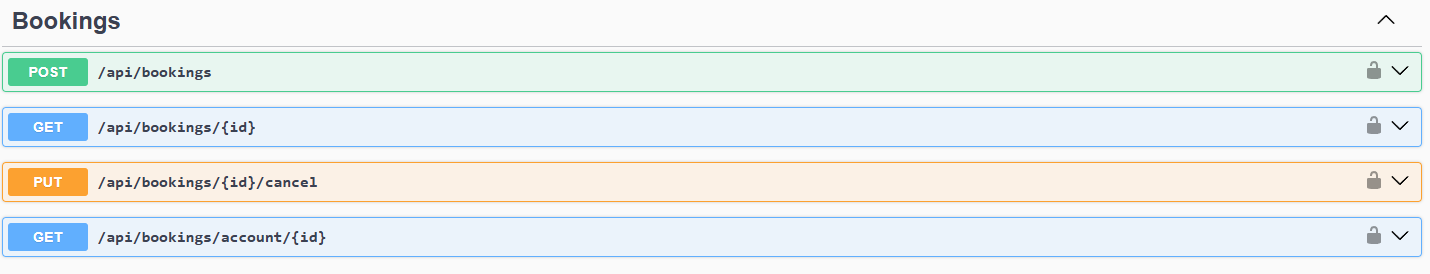
\includegraphics[width=\textwidth]{image/swagger/bookings.png}
  \caption{Swagger UI --- nhóm endpoint Bookings}\label{fig:sw_bookings}
\end{figure}

\begin{figure}[H]
  \centering
  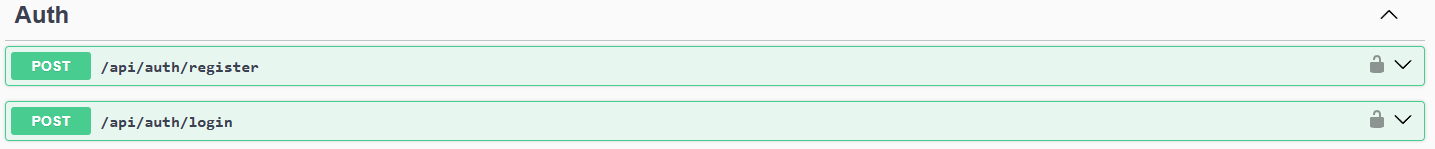
\includegraphics[width=\textwidth]{image/swagger/auth.png}
  \caption{Swagger UI --- nhóm endpoint Auth}\label{fig:sw_auth}
\end{figure}

\begin{figure}[H]
  \centering
  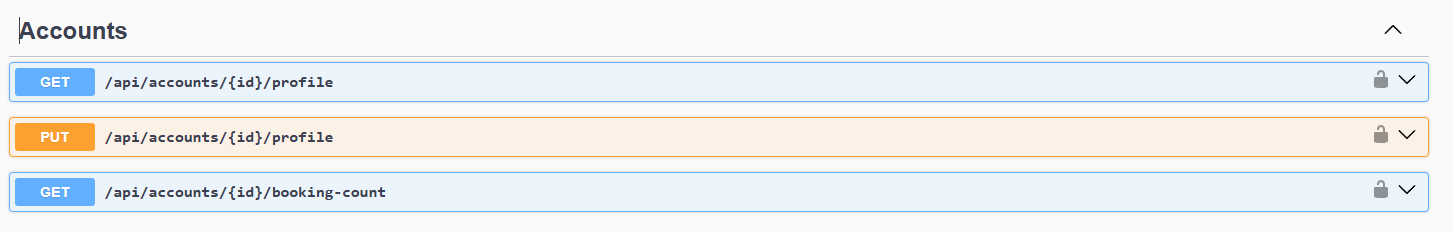
\includegraphics[width=\textwidth]{image/swagger/accounts.png}
  \caption{Swagger UI --- nhóm endpoint Accounts}\label{fig:sw_accounts}
\end{figure}

\begin{figure}[H]
  \centering
  
\includegraphics[width=\textwidth]{image/swagger/employees.png}
  \caption{Swagger UI --- nhóm endpoint Employees}\label{fig:sw_employees}
\end{figure}

\begin{figure}[H]
  \centering
  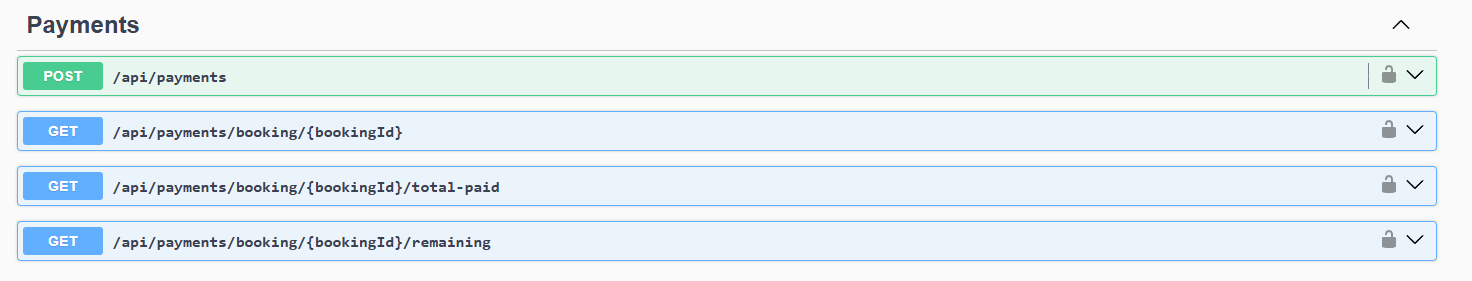
\includegraphics[width=\textwidth]{image/swagger/payments.png}
  \caption{Swagger UI --- nhóm endpoint Payments}\label{fig:sw_payments}
\end{figure}

\begin{figure}[H]
  \centering
  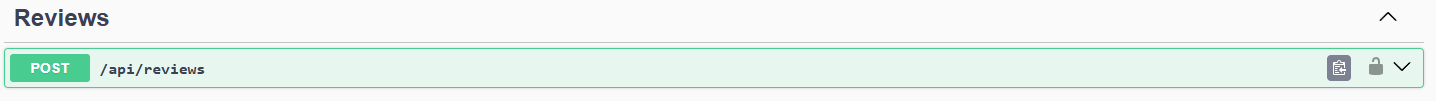
\includegraphics[width=\textwidth]{image/swagger/reviews.png}
  \caption{Swagger UI --- nhóm endpoint Reviews}\label{fig:sw_reviews}
\end{figure}

\begin{figure}[H]
  \centering
  
\includegraphics[width=\textwidth]{image/swagger/categories.png}
  \caption{Swagger UI --- nhóm endpoint Categories}\label{fig:sw_categories}
\end{figure}

\begin{figure}[H]
  \centering
  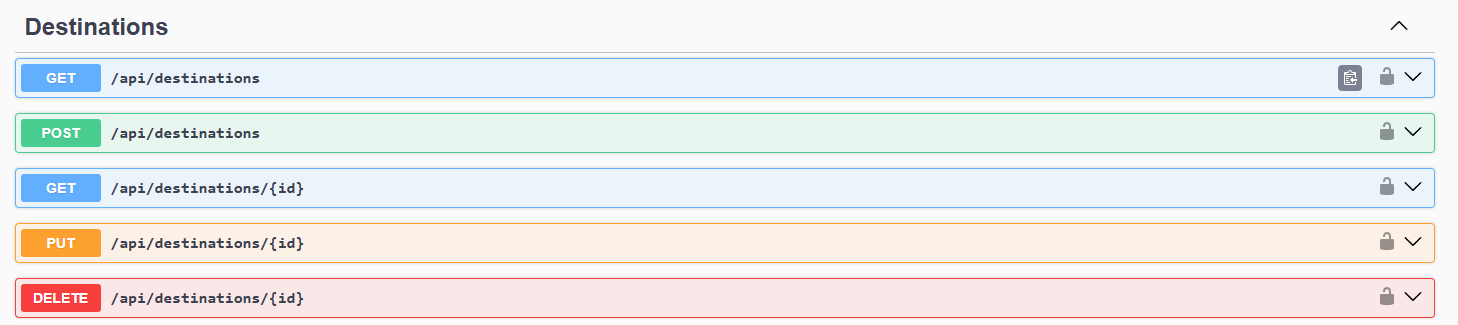
\includegraphics[width=\textwidth]{image/swagger/destinations.png}
  \caption{Swagger UI --- nhóm endpoint Destinations}\label{fig:sw_destinations}
\end{figure}

\begin{figure}[H]
  \centering
  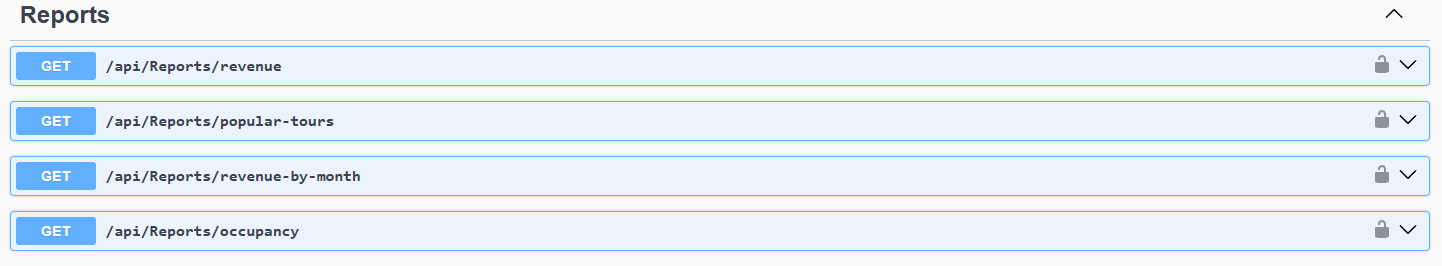
\includegraphics[width=\textwidth]{image/swagger/reports.png}
  \caption{Swagger UI --- nhóm endpoint Reports}\label{fig:sw_reports}
\end{figure}

% [TV4] Chụp màn hình Postman kết quả test (Collection Runner hoặc request/response),
%       lưu thành file rồi thay \framebox bên dưới.

\subsection{Kiểm thử API với Postman}\label{sub4.5.2}

Để đảm bảo tính chính xác và luồng hoạt động thực tế của hệ thống, các API được kiểm thử theo một kịch bản hoàn chỉnh trên Postman bao gồm 6 bước như sau:

\textbf{Bước 1: Auth — Đăng ký \& Đăng nhập} \\
Thực hiện tạo tài khoản mới (\texttt{POST /api/auth/register}) và đăng nhập (\texttt{POST /api/auth/login}) để lấy JWT token. Token này sẽ được gắn vào Header (\texttt{Authorization: Bearer <token>}) cho các bước tiếp theo.

\begin{figure}[H]
  \centering
  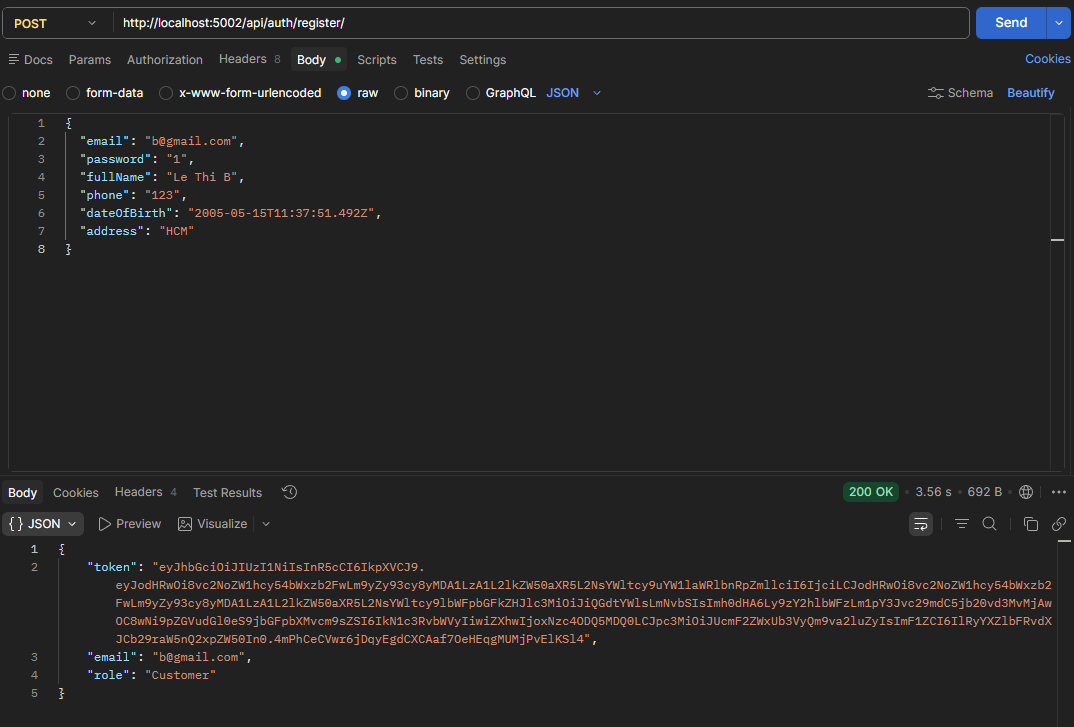
\includegraphics[width=0.8\textwidth]{image/postman/auth/register.png} \\[2ex]
  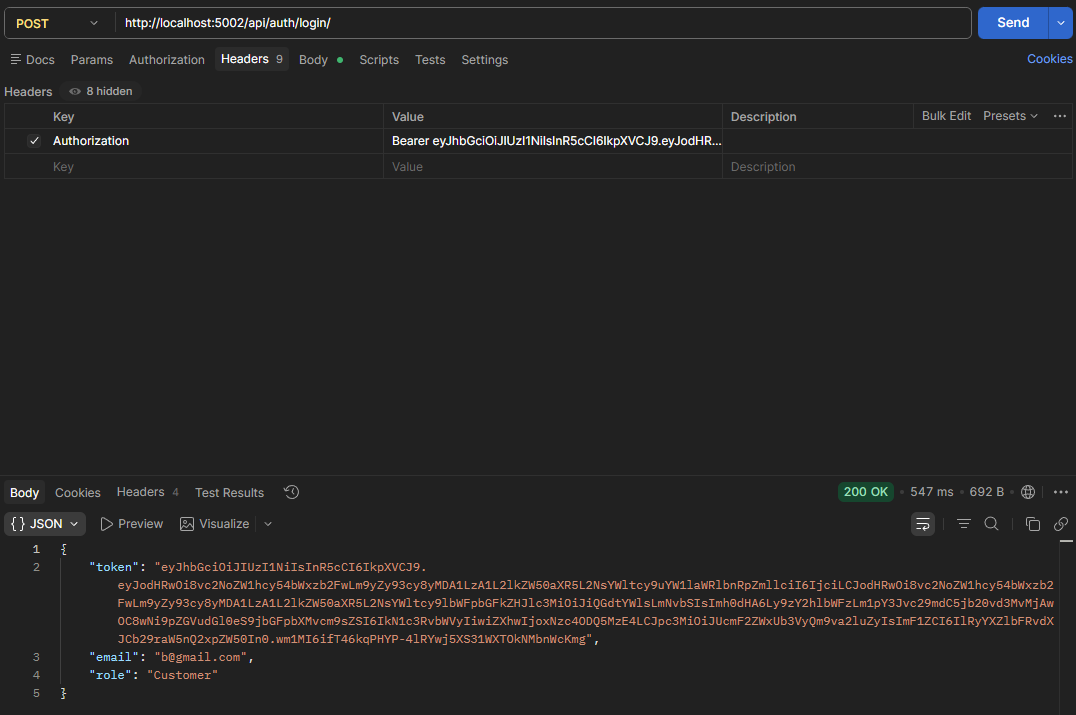
\includegraphics[width=0.8\textwidth]{image/postman/auth/login.png}
  \caption{Postman --- Bước 1: Đăng ký và Đăng nhập}\label{fig:pm_auth}
\end{figure}

\textbf{Bước 2: Setup dữ liệu nền (Quyền Admin)} \\
Sử dụng token của Admin để khởi tạo các dữ liệu cơ sở: Loại tour (\texttt{/api/categories}), Điểm đến (\texttt{/api/destinations}), Hướng dẫn viên (\texttt{/api/employees}), sau đó tạo Tour (\texttt{/api/tours}) và Lịch khởi hành (\texttt{/api/schedules}).

\begin{figure}[H]
  \centering
  
\includegraphics[width=0.7\textwidth]{image/postman/post_data/categories.png} \\[2ex]
  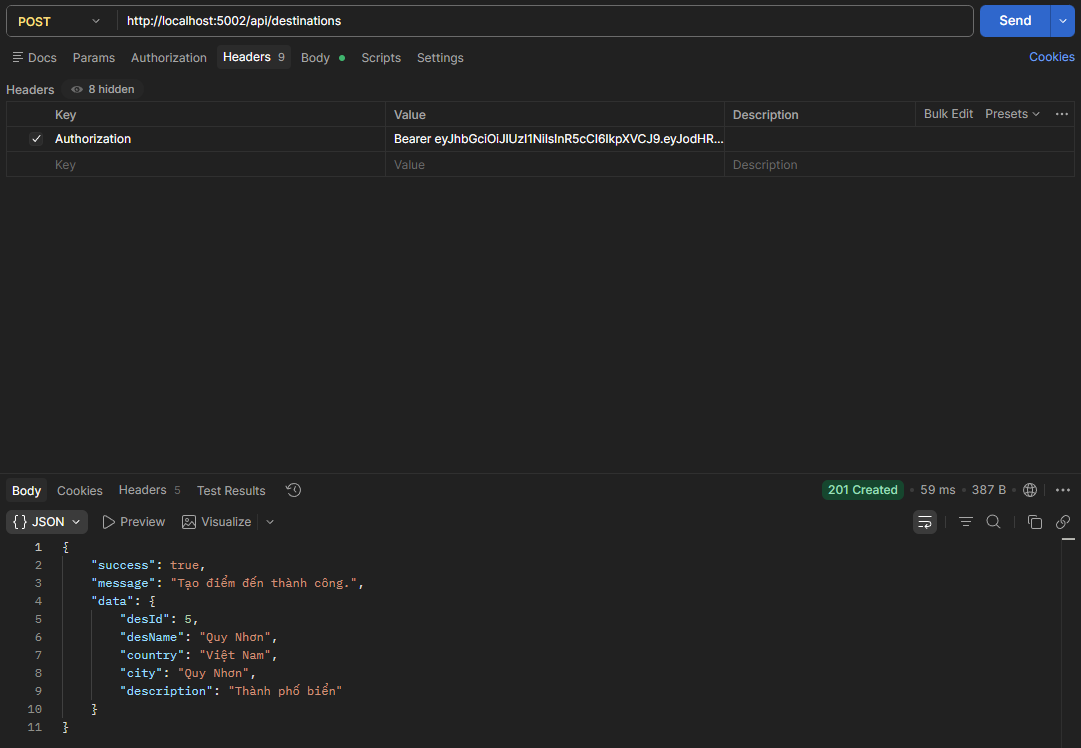
\includegraphics[width=0.7\textwidth]{image/postman/post_data/des.png} \\[2ex]
  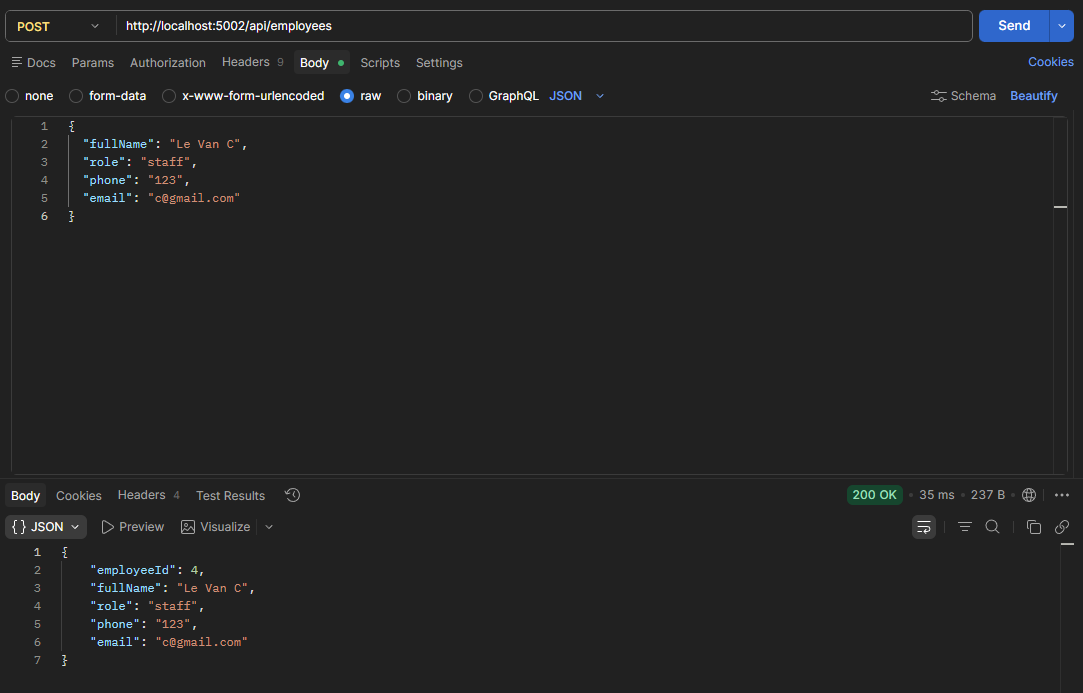
\includegraphics[width=0.7\textwidth]{image/postman/post_data/employees.png}
  \caption{Postman --- Bước 2: Khởi tạo dữ liệu nền (Admin)}\label{fig:pm_setup}
\end{figure}

\textbf{Bước 3: Xem danh sách (Public)} \\
Kiểm tra các endpoint không yêu cầu xác thực. Khách hàng xem danh sách tour, tìm kiếm nâng cao (\texttt{/api/tours/search}), xem tour phổ biến, chi tiết tour và lịch trình cụ thể.

\begin{figure}[H]
  \centering
  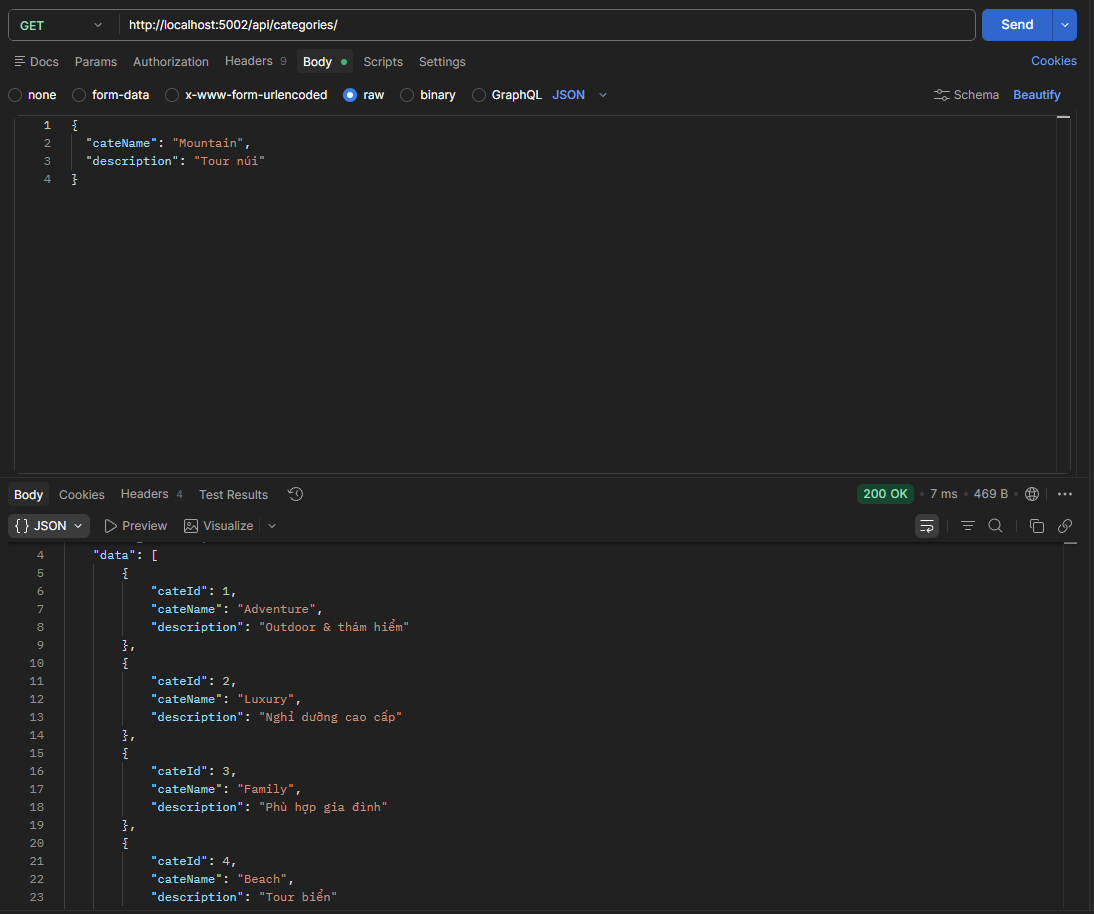
\includegraphics[width=0.75\textwidth]{image/postman/get_data/categories.png} \\[2ex]
  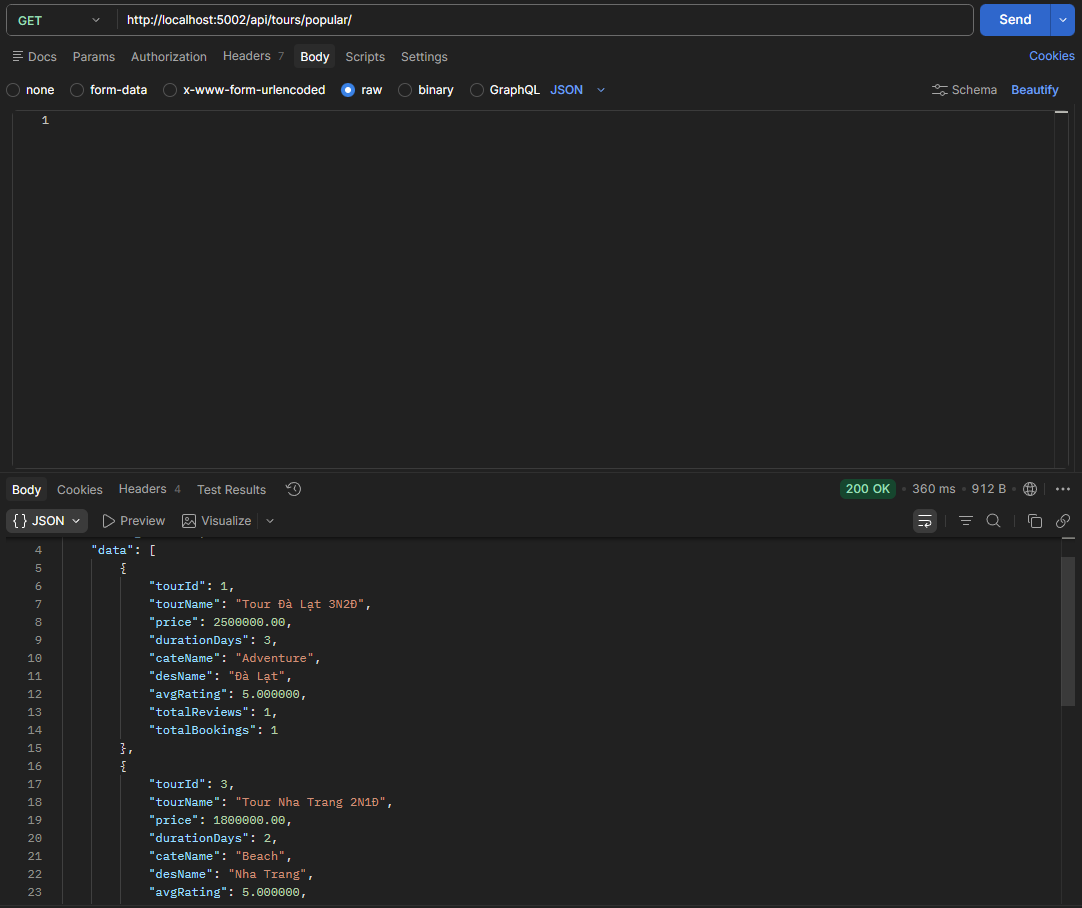
\includegraphics[width=0.75\textwidth]{image/postman/get_data/tours_popular.png}
  \caption{Postman --- Bước 3: Tra cứu và tìm kiếm tour}\label{fig:pm_public}
\end{figure}

\textbf{Bước 4: Đặt tour \& Thanh toán (Quyền Customer)} \\
Sử dụng token của Khách hàng để thực hiện quy trình đặt tour (\texttt{POST /api/bookings}), kiểm tra lại chi tiết booking, thanh toán (\texttt{POST /api/payments}) và kiểm tra số tiền đã trả/còn lại.

\begin{figure}[H]
  \centering
  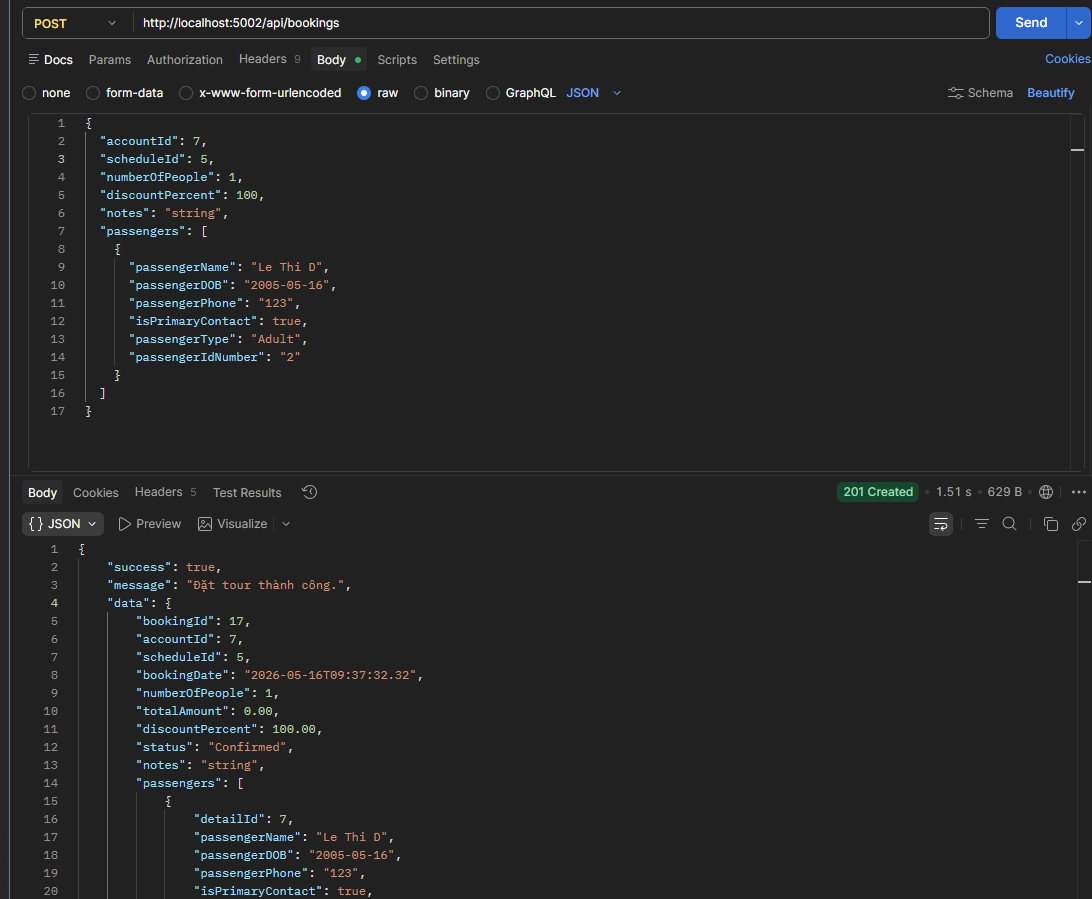
\includegraphics[width=0.70\textwidth]{image/postman/booking_payment/post_booking.png} \\[2ex]
  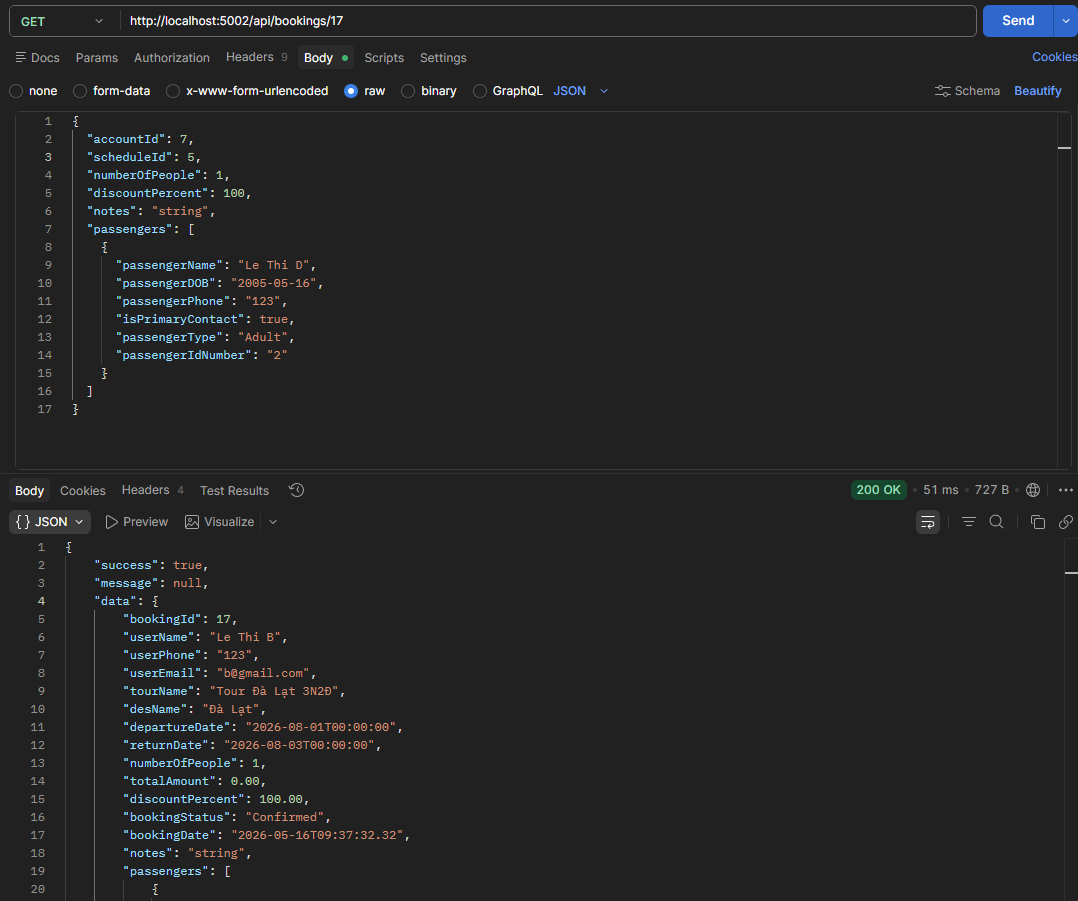
\includegraphics[width=0.70\textwidth]{image/postman/booking_payment/get_booking_id.png}
  \caption{Postman --- Bước 4: Đặt tour (1)}
\end{figure}

\begin{figure}[H]
  \centering
  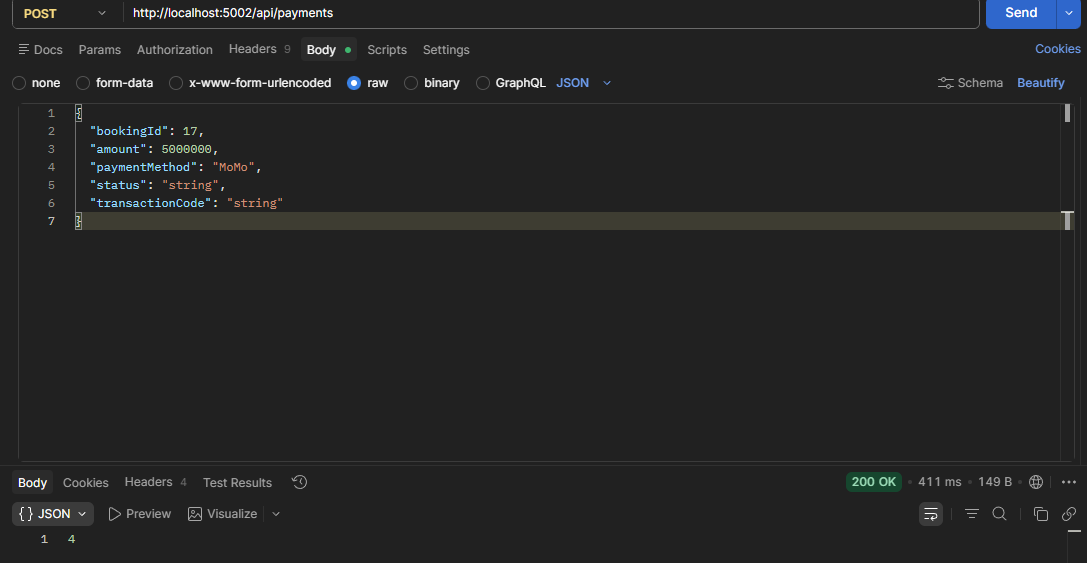
\includegraphics[width=0.70\textwidth]{image/postman/booking_payment/post_payment.png} \\[2ex]
  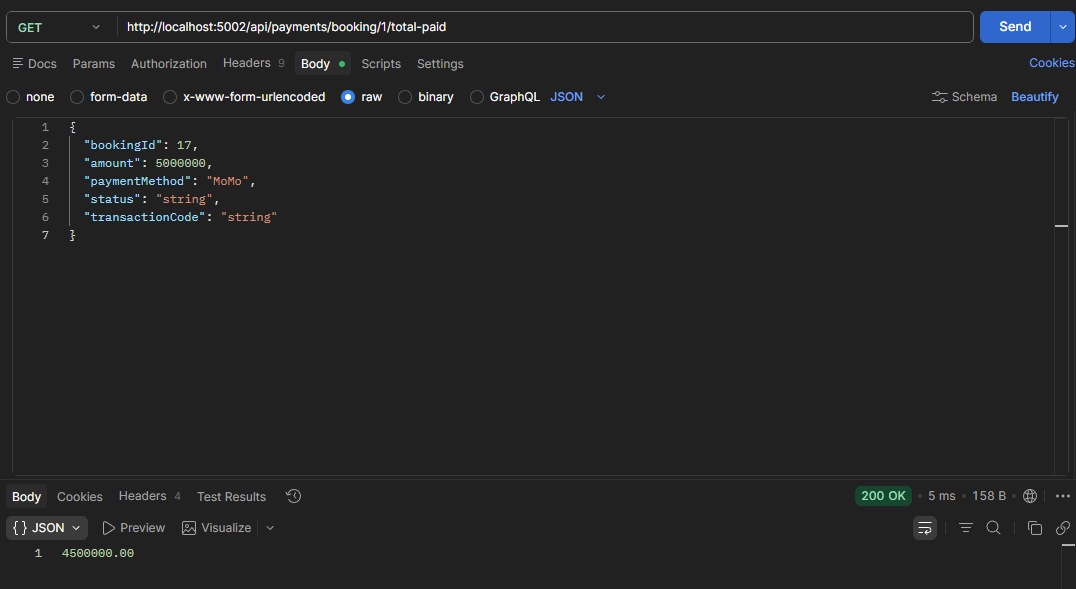
\includegraphics[width=0.70\textwidth]{image/postman/booking_payment/get_total_paid.png} \\[2ex]
  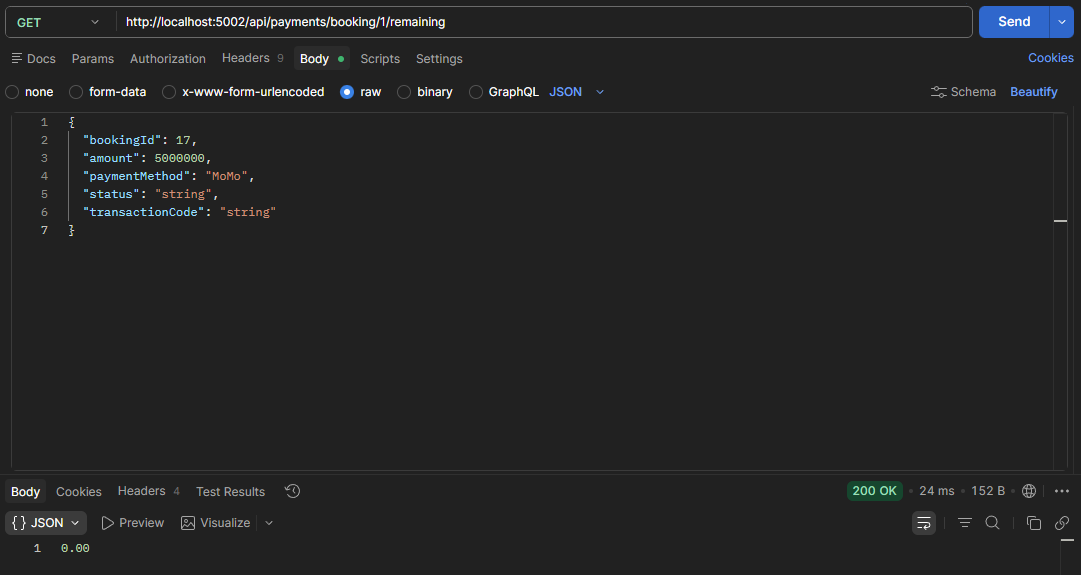
\includegraphics[width=0.70\textwidth]{image/postman/booking_payment/get_remaining.png}
  \caption{Postman --- Bước 4: Thanh toán và kiểm tra (2)}\label{fig:pm_booking}
\end{figure}

\textbf{Bước 5: Sau khi hoàn thành tour} \\
Khách hàng thực hiện đánh giá tour (\texttt{POST /api/reviews}), xem lại lịch sử booking của bản thân (\texttt{GET /api/bookings/account/\{id\}}) hoặc test chức năng hủy booking nếu chưa khởi hành.

\begin{figure}[H]
  \centering
  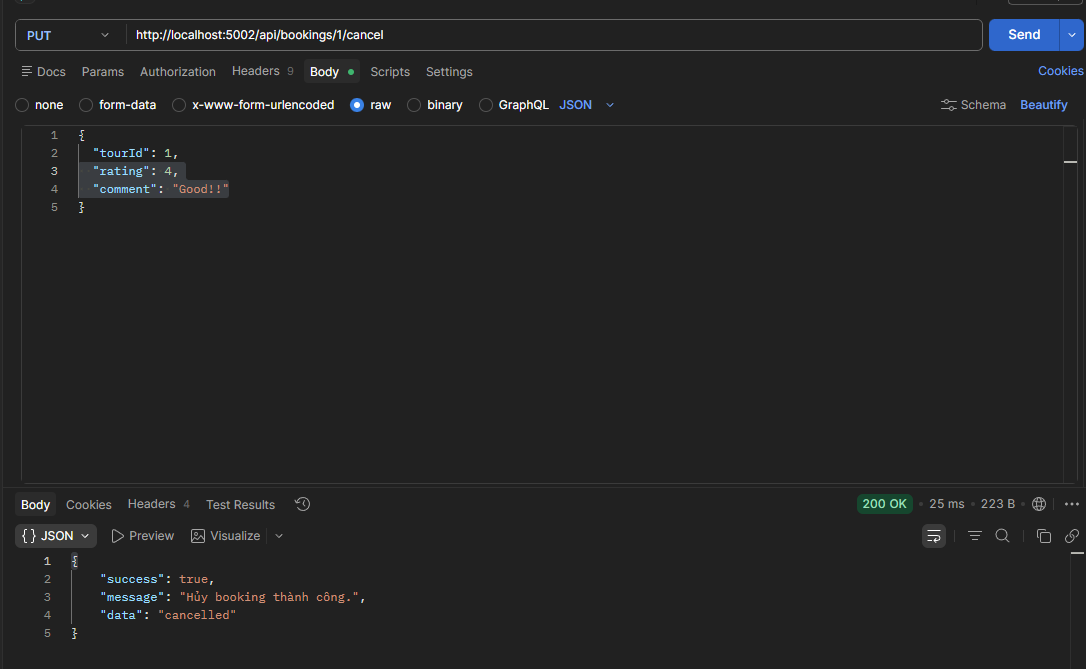
\includegraphics[width=\textwidth]{image/postman/tour_done/cancel.png} \\[2ex]
  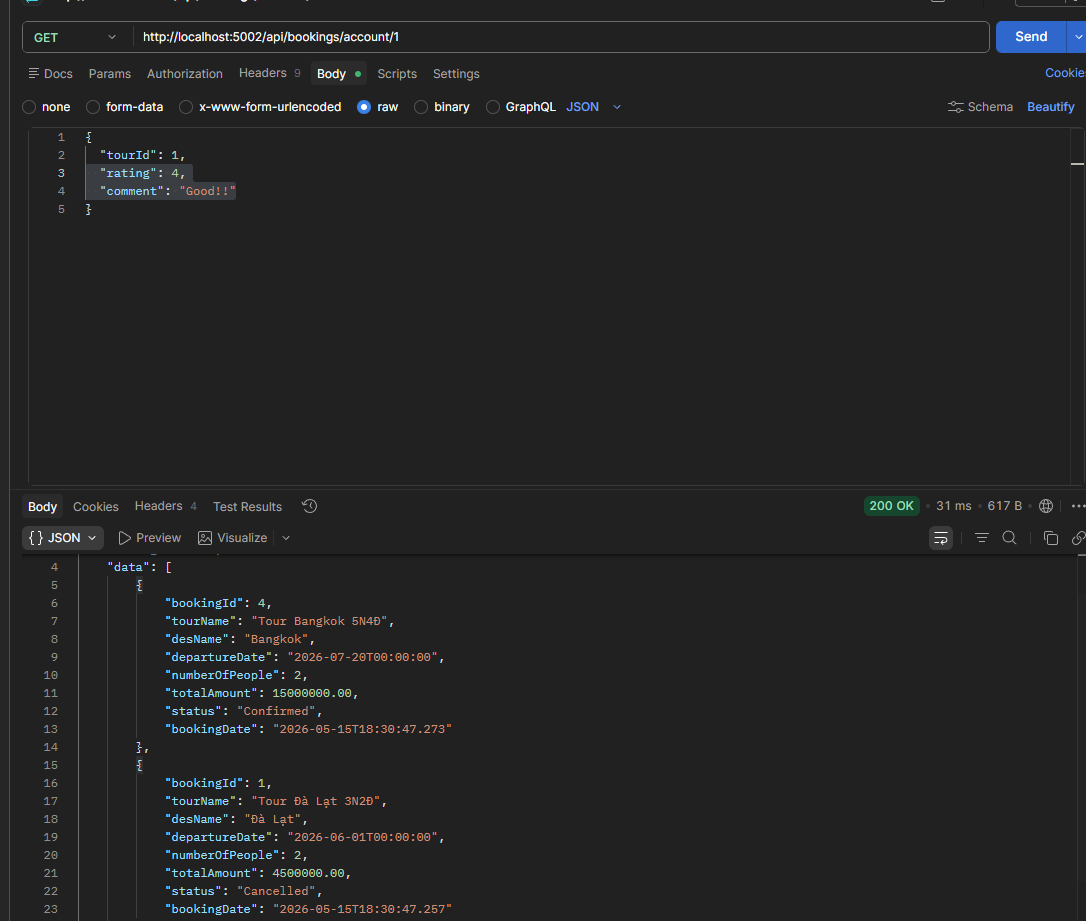
\includegraphics[width=\textwidth]{image/postman/tour_done/get_booking_history.png} \\[2ex]
  \caption{Postman --- Bước 5: Thực hiện hủy và lịch sử booking}\label{fig:pm_after}
\end{figure}

\textbf{Bước 6: Báo cáo thống kê (Quyền Admin)} \\
Admin gọi các endpoint báo cáo để truy xuất doanh thu, danh sách tour phổ biến, doanh thu theo tháng và tỷ lệ lấp đầy chỗ nhằm phục vụ Dashboard.

\begin{figure}[H]
  \centering
  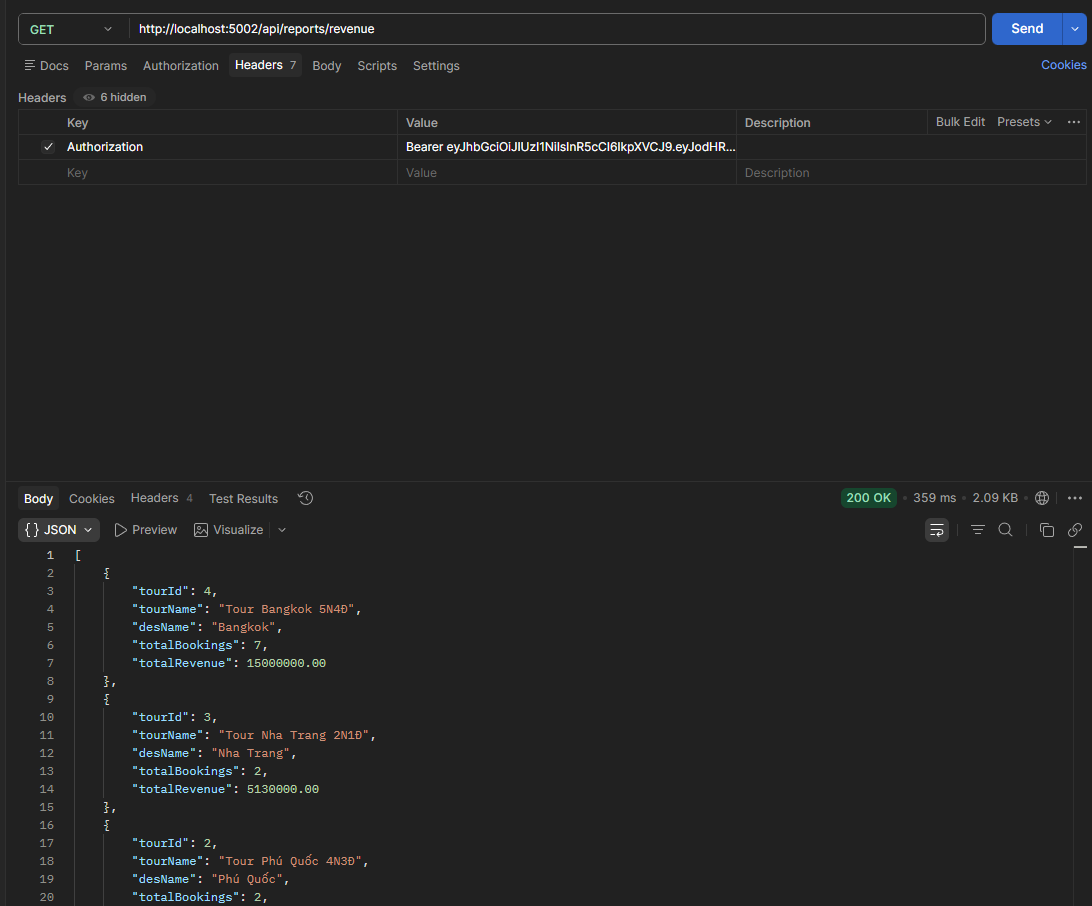
\includegraphics[width=0.9\textwidth]{image/postman/reports/get_revenue.png}
  \caption{Postman --- Báo cáo doanh thu}\label{fig:pm_rev}
\end{figure}

\begin{figure}[H]
  \centering
  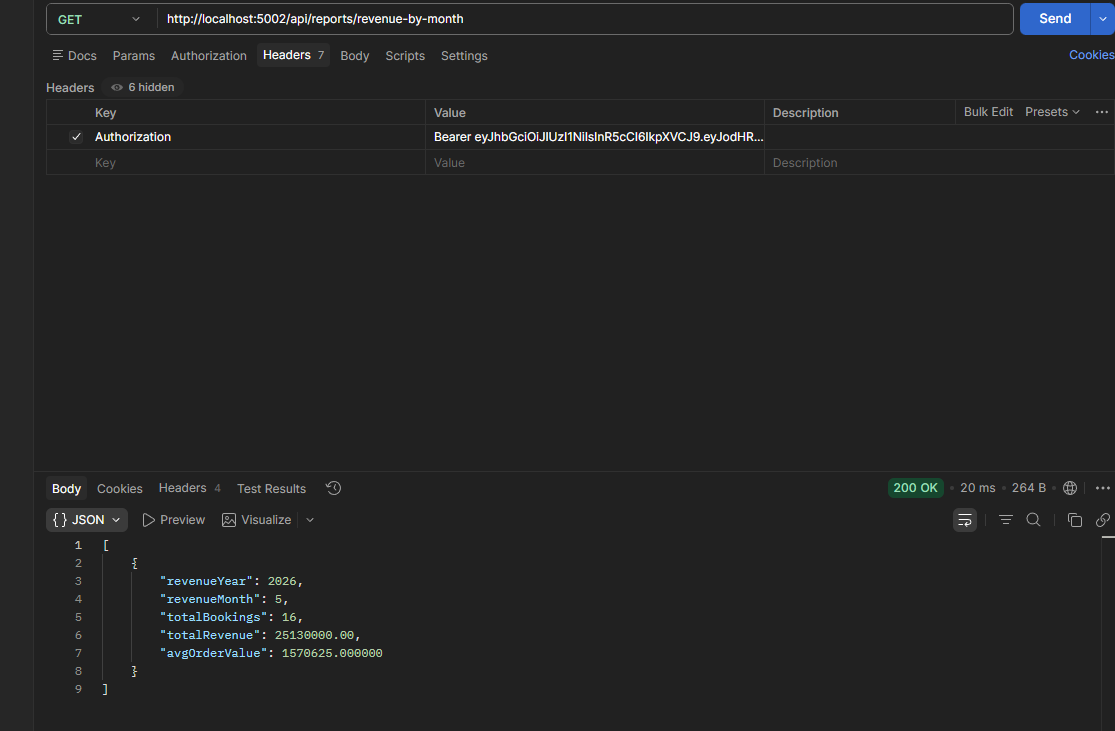
\includegraphics[width=0.9\textwidth]{image/postman/reports/get_revenue_monthly.png}
  \caption{Postman --- Báo cáo doanh thu theo tháng}\label{fig:pm_rev_month}
\end{figure}

\begin{figure}[H]
  \centering
  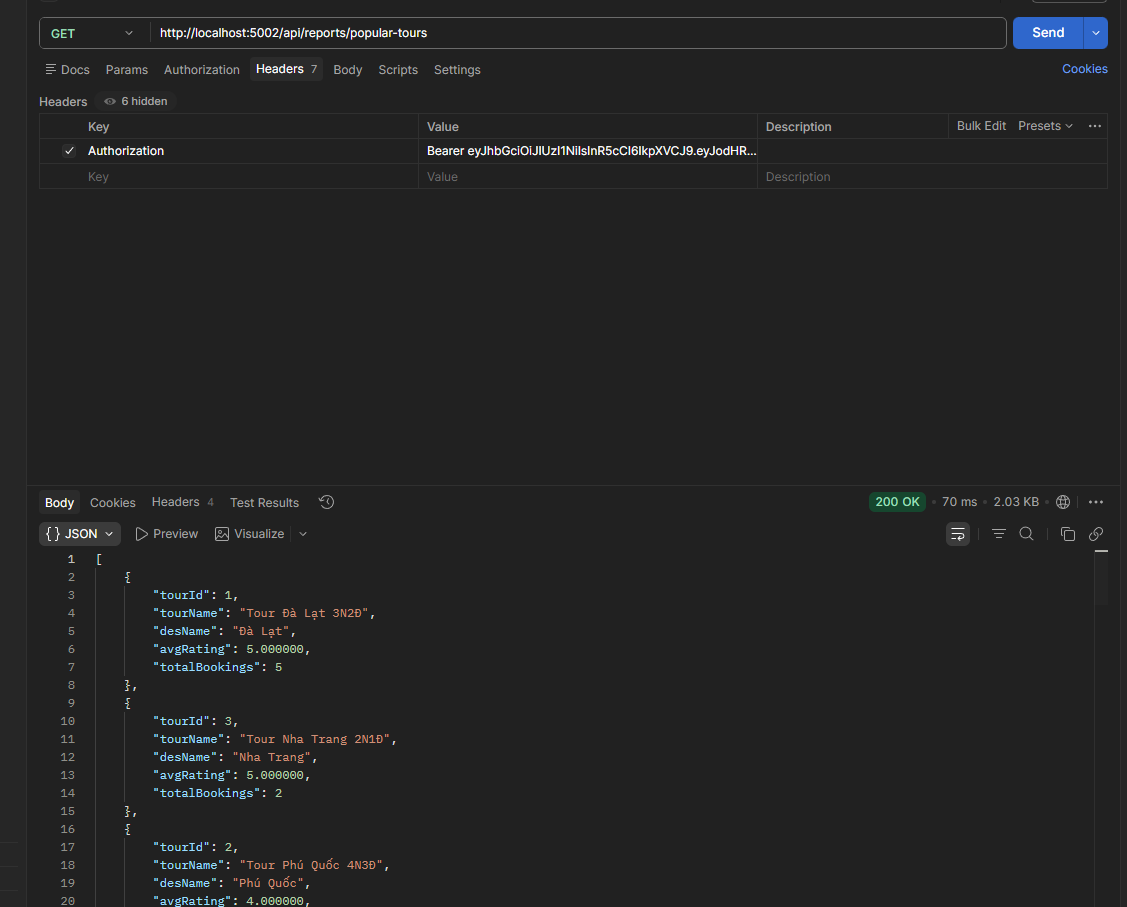
\includegraphics[width=0.9\textwidth]{image/postman/reports/get_popular_tours.png}
  \caption{Postman --- Thống kê các tour phổ biến}\label{fig:pm_pop_tours}
\end{figure}

\begin{figure}[H]
  \centering
  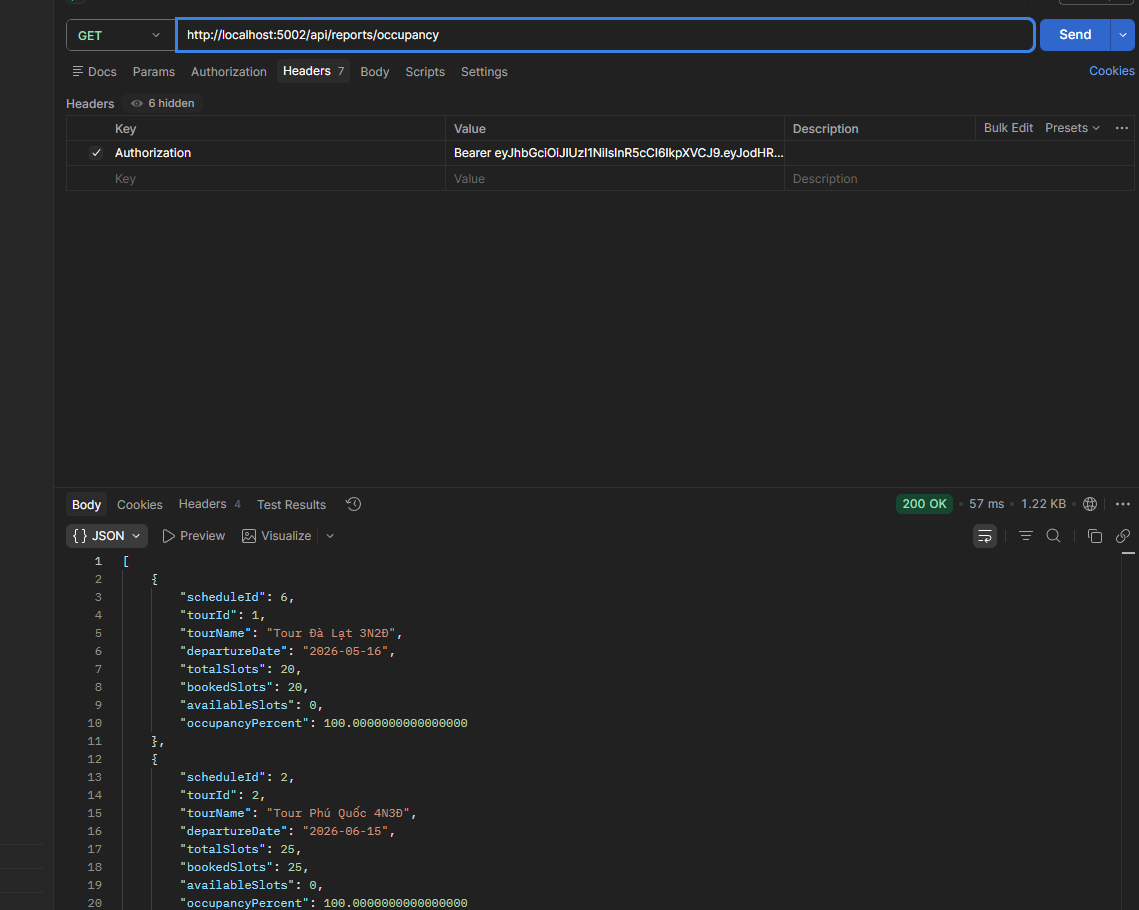
\includegraphics[width=0.9\textwidth]{image/postman/reports/get_occupancy.png}
  \caption{Postman --- Thống kê tỷ lệ lấp đầy (Occupancy)}\label{fig:pm_occupancy}
\end{figure}
\section{Dashboard}\label{Sec4.6}

% [TV4/TV5] Nếu nhóm xây dựng giao diện Frontend/Dashboard,
% mô tả ngắn công nghệ sử dụng và chèn screenshot.
% Nếu không có, có thể xóa section này.

Dashboard Admin được xây dựng bằng \textbf{Angular 17} (Standalone Components)
kết hợp thư viện \textbf{Chart.js} để trực quan hóa dữ liệu báo cáo.
Giao diện gồm ba thành phần chính: biểu đồ cột doanh thu theo tháng
(dữ liệu từ \texttt{sp\_RevenueReport} qua endpoint
\texttt{GET /api/reports/revenue-by-month}),
biểu đồ tròn tour phổ biến (\texttt{vw\_PopularTours}
qua \texttt{GET /api/reports/popular-tours}),
và bộ thẻ tóm tắt tổng doanh thu / tổng booking / tỷ lệ lấp đầy
(\texttt{GET /api/reports/occupancy}).
JWT Interceptor tự động đính token vào mọi request; Auth Guard
bảo vệ route \texttt{/dashboard} --- chỉ tài khoản Admin mới truy cập được.

\begin{figure}[H]
  \centering
  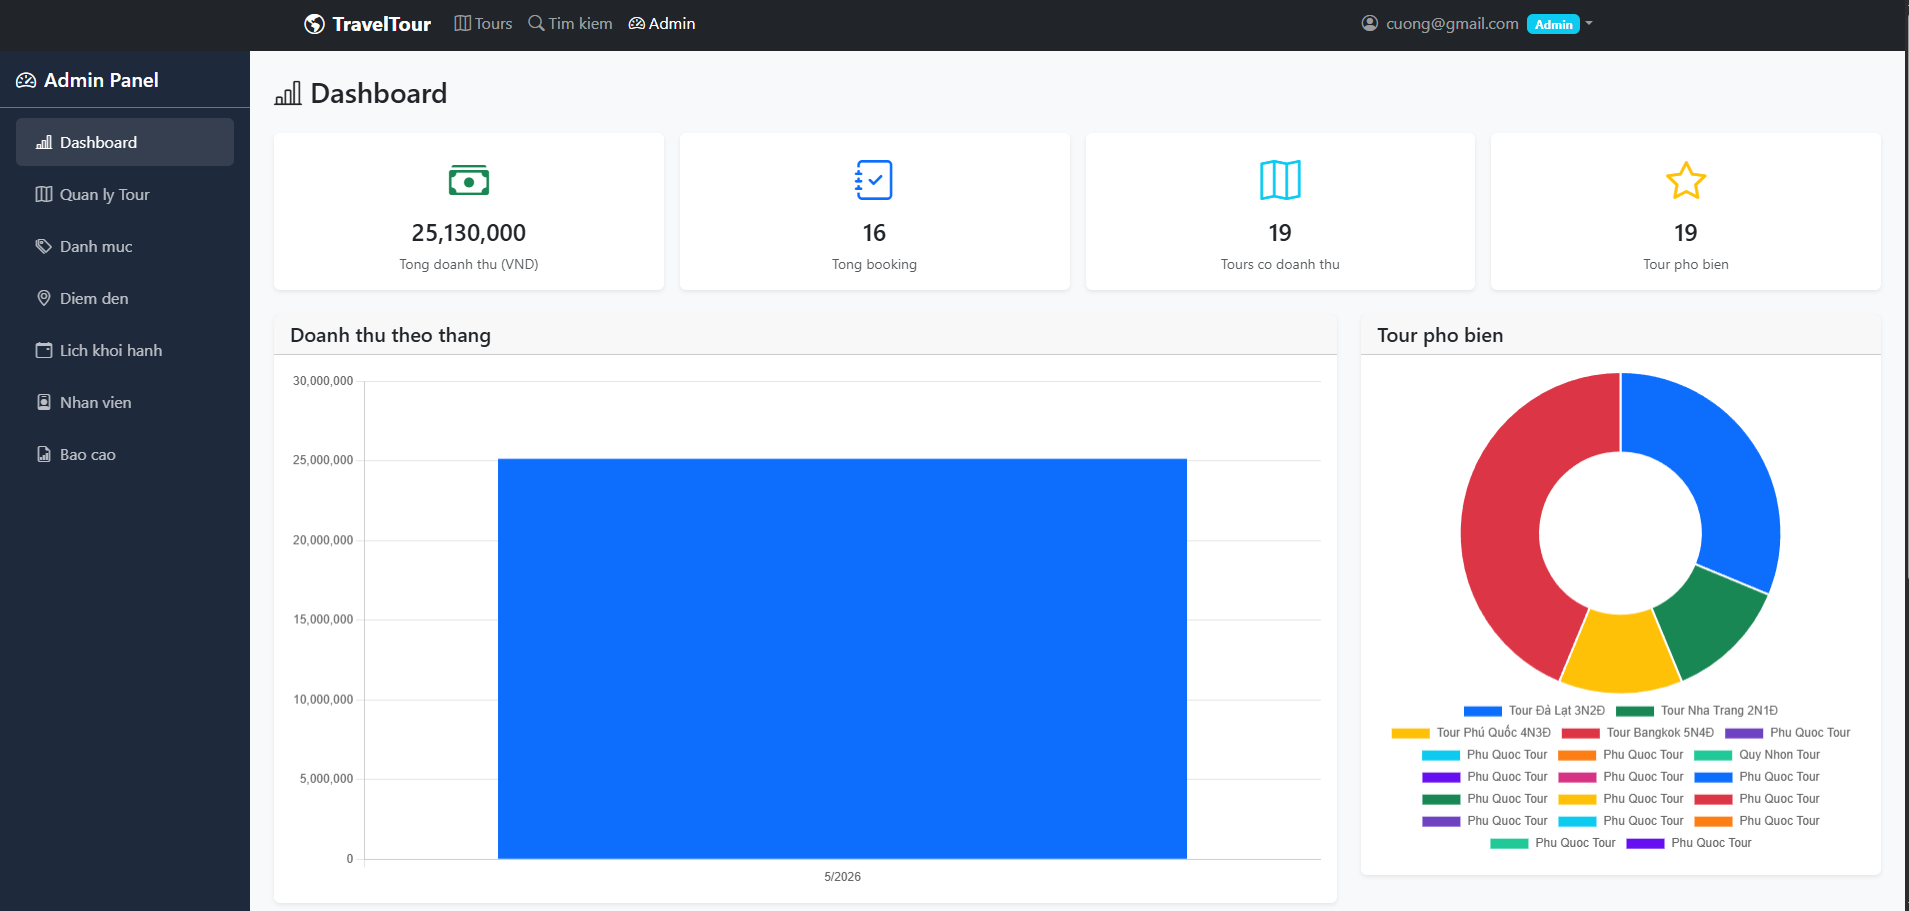
\includegraphics[width=\textwidth]{image/dashboard_admin.png} \\[2ex]
  \caption{Giao diện Dashboard báo cáo}\label{fig:dashboard}
\end{figure}